\documentclass{article}
\usepackage{pgfplots}
\pgfplotsset{compat=1.17}
\usepackage{graphicx}



\begin{document}
\title{Calculus III Homework 3 Question 2}


Find a vector a with representation given by the directed line segment AB. Draw AB

$
   5: A(-1, 1), B(3,2): AB = <3-(-1),2-1 > = <4,1>
$



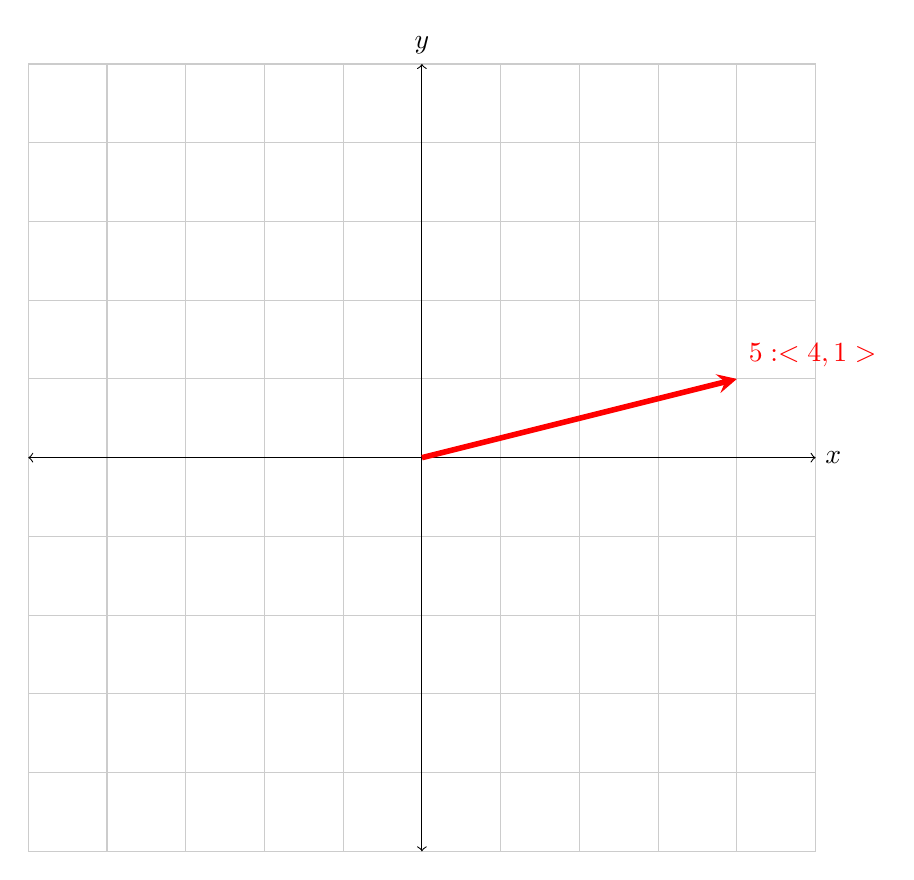
\begin{tikzpicture}
  \draw[thin,gray!40] (-5,-5) grid (5,5);
  \draw[<->] (-5,0)--(5,0) node[right]{$x$};
  \draw[<->] (0,-5)--(0,5) node[above]{$y$};
  \draw[line width=2pt,red,-stealth](0,0)--(4,1) node[anchor=south west]{${5: <4,1>}$};
\end{tikzpicture}

\pagebreak
$6: A(-4,-1), B(1,2) : AB = <1-(-4),2-(-1))> = <5,3>$

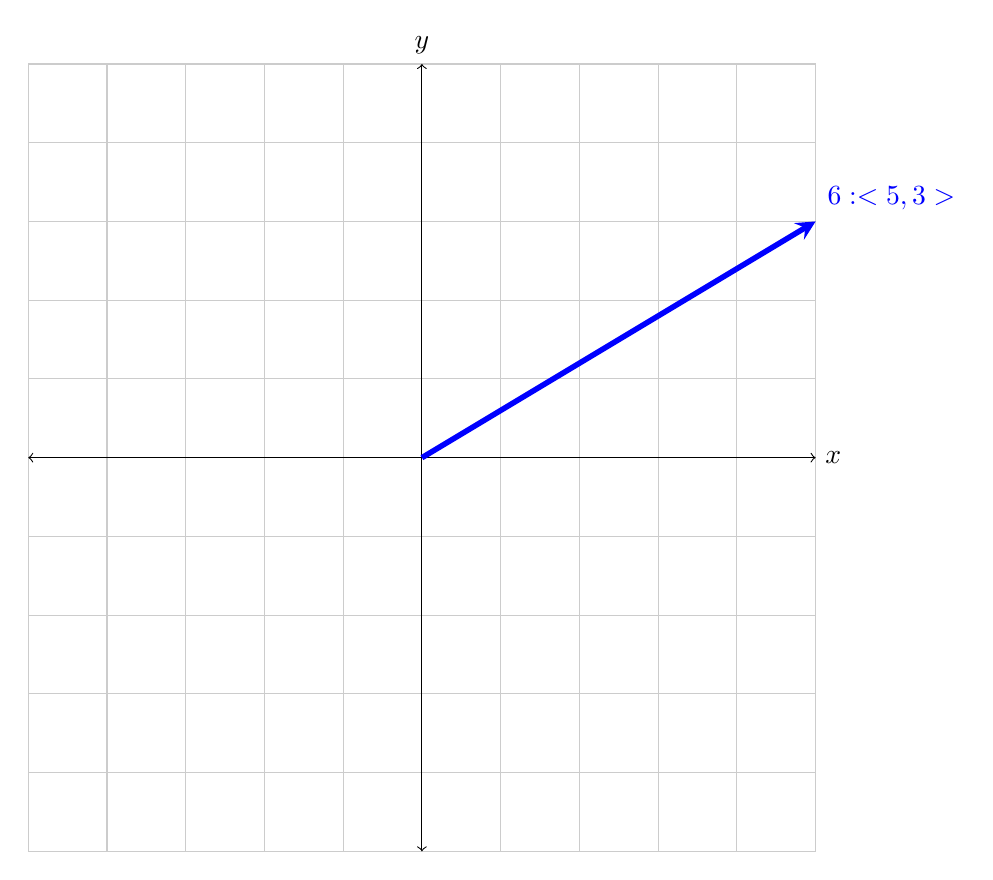
\begin{tikzpicture}
  \draw[thin,gray!40] (-5,-5) grid (5,5);
  \draw[<->] (-5,0)--(5,0) node[right]{$x$};
  \draw[<->] (0,-5)--(0,5) node[above]{$y$};
  \draw[line width=2pt,blue,-stealth](0,0)--(5,3) node[anchor=south west]{${6: <5,3>}$};
\end{tikzpicture}

\pagebreak
$
7: A(0,3,1), B(2,3,-1) : AB = <2-0,3-3,(-1)-1> = <2,0,-2>
$
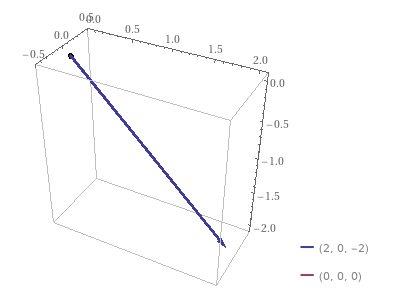
\includegraphics{image.png}
\\

\pagebreak
$
8: A(4,0,-2), B(4,2,1) : AB = <4-4,2-0,1-(-2)> = <0,2,3>
$
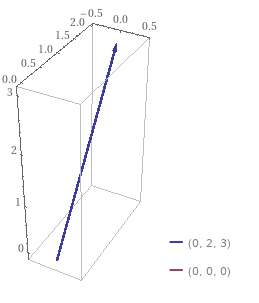
\includegraphics{graph 023.png}
\end{document}